\documentclass{book}
\usepackage{amssymb,latexsym,color,amsthm}

%allows for comment blocks and verbatim sections
\usepackage{verbatim}

%preserves tabs in verbatim sections. Good for including source code in documents.
\usepackage{moreverb}

%The following are for the example boxes
\usepackage{graphicx}
\definecolor{Dark}{gray}{.20}
\definecolor{Light}{gray}{.80}
\newcommand{\examplein}[1]{\begin{center} \colorbox{Dark}{\textcolor{white}{#1}} \end{center}}
\newcommand{\exampleout}[1]{\begin{center} \colorbox{Light}{\textcolor{black}{#1}} \end{center}}

%This is how I made the example environment
\newtheorem{ex}{Exercise}[chapter]

\begin{document}

\title{An intro to writing workshops for mentoring program in latex}
\author{Brandon Tarquinio}

\maketitle
\tableofcontents
\newpage
\chapter{The Basics}
The above line\footnote{When I mention ``lines" (also note how I just qoated that string) I am assuming you are reading the template.tex file not the compiled template.pdf file} will place the header for the first chapter and add the entry to the table of contents. This text will appear after the header ``The Basics" but before the first section. You can use this for introductions to chapters. 
\section{Here is basic text and footnotes}
Here is some text!\footnote{And here is a footnote}
\subsection{Subsections}
This is how you make a subsection.


\section{Examples}
This section regards example layouts.
\subsection{Basics}
It's optional to start with a motivation. Then give the general form of what you want to discuss. Follow that by example of what they should enter using this:
\examplein{head -v --lines=20 myfile}
Then use the other colour box to show results like this:
\exampleout{here is the output!}
If you decide you need more types of boxes then see the preamble of this document where I defined these commands.
\subsection{exercises and lists}
\begin{ex} 
	You can run any latex commands inside the ex environment and it will display in italics. For example you can use the examplein and exampleout command like before:
	\examplein{do this}
	\exampleout{See this?}
	Some text and examplein and exampleout suffices for smaller exercies but for larger ones lists will help to show the steps. You can make numbered lists with the enumerate environment like this:
\begin{enumerate}
	\item Here is my first item. \examplein{it contains an example}
	\item See how this works?
\end{enumerate}
	Or instead you could make bullet point lists with the itemize environment like this:
	\begin{itemize}
		\item Here is some text.
		\item and here is some more.
	\end{itemize}
	Also you can define your own list headers like this
	\begin{description}
		\item[First.] here is some text.
		\item[And another style] \hfill \\
			Here is indented text on next line.
	\end{description}
\end{ex}
Of course those lists can also be made outside examples.

\subsection{Inserting an image}
%Remember this is how you make comments!
\newpage
Note my use of the newpage command to cause page breaks. This can come in handy when you don't want your example to be half on one page and half on the other. Or in this case I used it so the Image and text would appear correctly. Try commenting out the newpage and see what happens. 

Here is how I can insert an Image: \\
\begin{figure}[ht!]
	\centering
	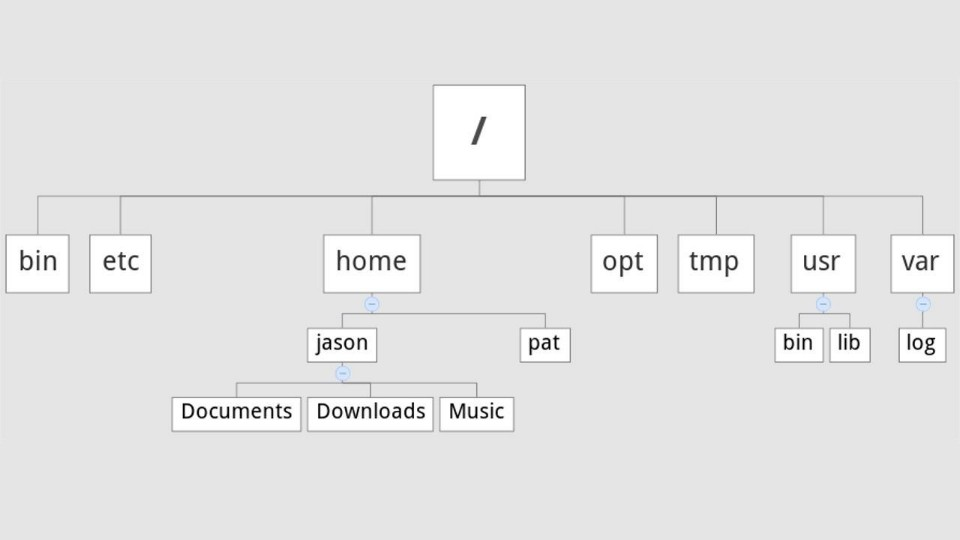
\includegraphics[width=90mm]{linux-directory-tree.jpg}
	\caption{An Example Linux Directory Tree.} 
\end{figure}
Note: if you make images then give yourself credit! Add a entry to the reference page and either the caption or surrounding text. Even more importantly cite anything you grab from the internet! \\
Note2: The image file needs to be in the same folder when you compile or you will get an error. Alternatively you can give the absolute path name in the argument. \\

\subsection{Final notes on examples}
	I think it is very helpful to explain what the commands stand for if they do have a translation. For example if I was writing the vim workshop I would probably have the following lines: \\
	When we want to save or \textbf{w}rite our file we enter the the following in command mode:
	\examplein{:w}
	We can exit or \textbf{q}uit the program with the following:
	\examplein{:q}

\subsection{How to write code in latex}
\begin{verbatimtab}
	#include <stdio.h>

	int main() {
		printf("Hello World!");
	}
\end{verbatimtab}
Notice in the above example that everything was put in the pdf exactly like it was typed. No need to escape the escape characters or mess with indentation. It all just works!

\chapter{Another Chapter}
And this is how we make another chapter! I think you guys have got it by this point. Review the end of this document to see how I made the appendices. I would recommend making at least two: the first for all the code you use and another for a quick reference or glossery of the commands and terms you used in the workshop. Also take a look at how I used the bibliography to cite my image. Remember that if you copy any text or borrow to heavily from other resources you should also cite them. Doesn't need to be MLA or anything, just give credit when credit is due. \\

Thanks again everyone!

\newpage
\appendix
\section{\\Runnable Code from Examples} \label{App:AppendixA}
% the \\ insures the section title is centered below the phrase: AppendixA
The below code was tested using by being compiled using $gcc$ and then ran on Linux x86\_64: 
\begin{verbatimtab}
#include <stdio.h>
#include <stdlib.h>
#include <string.h>

char *foo(){
	int a = 5;
	char *b = "Let it be";
	char *c = "leed";
	int size_b = strlen(b);
	int size_c = strlen(c);
	char *ret_buf = (char *)malloc(size_b + size_c);
	int i;
	for (i = 0; i < size_b - 1; i++){
	 	ret_buf[i] = b[i];
	}
	for (i = 0; i < size_c; i++){
		ret_buf[i+size_b-1] = c[i];	
	}
	return ret_buf;
}

int main() {
	printf("%s", foo());	
}
\end{verbatimtab}

\newpage
\section{\\Quick Reference} \label{App:AppendixB}
% the \\ insures the section title is centered below the phrase: Appendix B

Make a table of the highlights here.

\newpage
\begin{thebibliography}{10}

	\bibitem{Figure 1} Figure 1 found at http://www.linuxtrainingacademy.com/wp-content/uploads/2014/03/linux-directory-tree.jpg \\

\end{thebibliography}
\end{document}
